%%%%%%%%%%%%%%%%%%%%%%%%%%%%%%%%%%%%%%%%%%%%%%%%%%%%%%%%%%%%%%%%%%%%%%%%%%%%%%%
\section{Pin-wise Spatial Homogenization Schemes}
\label{sec:pin-wise-shielding}
%%%%%%%%%%%%%%%%%%%%%%%%%%%%%%%%%%%%%%%%%%%%%%%%%%%%%%%%%%%%%%%%%%%%%%%%%%%%%%%

This paper introduces three spatial homogenization schemes to model inter-pin spatial self-shielding effects with varying degrees of granularity. Although all spatial zones may experience spatial self-shielding, this paper only models the spatial variation of MGXS in fissile regions and computes a single MGXS for each non-fissile material. Furthermore, this paper does not treat intra-pin spatial self-shielding (\textit{i.e.}, spatial self-shielding within a fuel pin) and instead assigns a single MGXS to all discretized spatial zones within each fuel pin. This constraint was made to directly isolate and quantify approximation errors resulting from inter-pin spatial self-shielding effects. The null, degenerate and Local Neighbor Symmetry spatial homogenization schemes are introduced in \autoref{subsec:homogenize-null}, \autoref{subsec:homogenize-degenerate} and \autoref{subsec:homogenize-lns}, respectively.


%%%%%%%%%%%%%%%%%%%%%%%%%%%%%%%%%%%%%%%%%%%%%%%%%%%%%%%%%%%%%%%%%%%%%%%%%%%%%%%
\subsection{Null Spatial Homogenization}
\label{subsec:homogenize-null}

The \textit{null} spatial homogenization scheme uses a single Monte Carlo calculation of the complete heterogeneous geometry to generate MGXS for each material. The spatially self-shielded flux is used to collapse the cross sections in each material with a unique isotopic composition. The null scheme does not account for spatial self-shielding effects experienced by different fuel pins filled by the same fuel composition, and instead averages these effects across the entire geometry. A single MGXS is employed in each instance of a material zone, such as a fuel pin replicated many times throughout a benchmark geometry. The null scheme serves as the base case in this paper to illustrate the approximation error which results when inter-pin spatial self-shielding effects are neglected, even when the exact flux from Monte Carlo is used to collapse continuous energy cross sections.


%%%%%%%%%%%%%%%%%%%%%%%%%%%%%%%%%%%%%%%%%%%%%%%%%%%%%%%%%%%%%%%%%%%%%%%%%%%%%%%
\subsection{Degenerate Spatial Homogenization}
\label{subsec:homogenize-degenerate}

The \textit{degenerate} spatial homogenization scheme accounts for spatial self-shielding effects experienced by each instance of each fuel pin throughout a heterogeneous geometry. Like the null scheme, a single MC calculation of the complete heterogeneous geometry is used to generate MGXS for all materials. Unlike the null scheme, the MGXS are tallied separately for each instance of fissile material zones. For example, if a heterogeneous benchmark includes $N$ fuel pins, then $N$ collections of MGXS are separately tabulated for each fuel pin instance. The degenerate scheme tallies different MGXS even if the isotopic compositions in the fuel pin instances are identical, since each instance may experience a different spatially self-shielded flux and hence have different MGXS. The degenerate scheme demonstrates the reduction in approximation error between multi-group and continuous energy transport methods that can be achieved when inter-pin spatial self-shielding effects are sufficiently modeled in MGXS.

%%%%%%%%%%%%%%%%%%%%%%%%%%%%%%%%%%%%%%%%%%%%%%%%%%%%%%%%%%%%%%%%%%%%%%%%%%%%%%%
\subsection{Local Neighbor Symmetry Spatial Homogenization}
\label{subsec:homogenize-lns}

The Local Neighbor Symmetry (LNS) spatial homogenization scheme uses a deterministic approach to spatially homogenize pin-wise MGXS based on an analysis of a reactor geometry. This approach is akin to geometric templates employed by lattice physics codes, such as CASMO \citep{edenius1995casmo}, to predict which groupings of pins are likely to experience similar spatial self-shielding effects. The goal of LNS homogenization is to reduce approximation error by accounting for spatial self-shielding effects on groupings of fuel pins with similar neighboring heterogeneities. This technique aims to compute MGXS which are nearly as accurate as those generated by degenerate homogenization, but require fewer MC particle histories to converge the tallies used to compute MGXS for each grouping of pins.

%The goal of LNS homogenization is to achieve the degenerate scheme's accuracy by modeling MGXS clustering, and approach the null scheme's tally convergence by homogenizing MGXS for each grouping of pins.

%The LNS algorithm analyzes a combinatorial geometry used to represent a reactor model and groups pins together based on their neighboring spatial zones.

%%%%%%%%%%%%%%%%%%%%%%%%%%%%%%%%%%%%%%%%%%%%%%%%%%%%%%%%%%%%%%%%%%%%%%%%%%%%%%%
\subsubsection{Local Neighbor Symmetry Identification}
\label{subsubsec:homogenize-lns}

The OpenCG code \citep{boyd2015opencg} was created to simplify the process of creating and transferring data mapped to combinatorial geometries for the OpenMC and OpenMOC neutron transport codes. One of the unique algorithms implemented in OpenCG is known as Local Neighbor Symmetry identification. The LNS algorithm systematically analyzes a combinatorial geometry (CG) tree data structure to identify neighbor cells, or pairs of cells which are adjacent to one another. The neighbor cells are assembled into a heuristic which groups similar spatial zones with common LNS identifiers. A brief overview of the algorithm is given here; the interested reader is referred to \citep{boyd2015opencg} for a more detailed discussion.

The LNS algorithm identifies the unique symmetry for the path to a region in a combinatorial geometry as described in \autoref{alg:lns}. The LNS algorithm performs a breadth-first search (BFS) to find neighbors on each level of the CG tree. For example, BFS is used to find neighbor cells for a particular cell within a universe. Similarly, BFS is used to find neighbor universes adjacent to a particular lattice cell. The neighbor cells and universes on each of the $k$ levels of a CG tree are connected to form a $k$-partite graph as depicted in \autoref{fig:lns-k-partite-graph}. Red nodes correspond to the universes/cells encapsulating a region of interest, green nodes correspond to the neighbors of that region, and gray nodes correspond to universes/cells which are not neighbors. Red and green nodes at each level are combined into an argument for a hash function to generate a LNS identifier (\textit{e.g.}, a non-negative integer) for the particular region represented by the path.

\begin{algorithm*}[h!]
\begin{algorithmic}[1]
\Procedure{computeNeighborSymmetry}{$path$}
    \State $G \gets \emptyset$ \Comment{Initialize empty set for graph}
    \State $k \gets$ \textbf{length}($path$) \Comment{Find number of independent sets}
    \For{$i := 1, k$}
        \If{\textbf{type}($path[i]$) \textbf{is} UNIVERSE}
            \State $G \gets G \cup \{path[i]\}$ \Comment{Append universe to graph}
        \ElsIf{\textbf{type}($path[i]$) \textbf{is} LATTICE}
            \State $N \gets$ \Call{BreadthFirstSearch}{$path[i]$} \Comment{Find lattice cell neighbors}
            \State $G \gets G \cup \{N\}$ \Comment{Append neighbors to graph}
        \ElsIf{\textbf{type}($path[i]$) \textbf{is} CELL}
            \State $N \gets$ \Call{BreadthFirstSearch}{$path[i]$} \Comment{Find cell neighbors}
            \State $G \gets G \cup \{N\}$ \Comment{Append neighbors to graph}
        \EndIf
    \EndFor
    \State \textbf{return} \Call{Hash}{$G$} \Comment{Return $k$-partite graph hash}
\EndProcedure
\caption{Local Neighbor Symmetry Identification}
\label{alg:lns}
\end{algorithmic}
\end{algorithm*}

\begin{figure*}[h!]
  \centering
  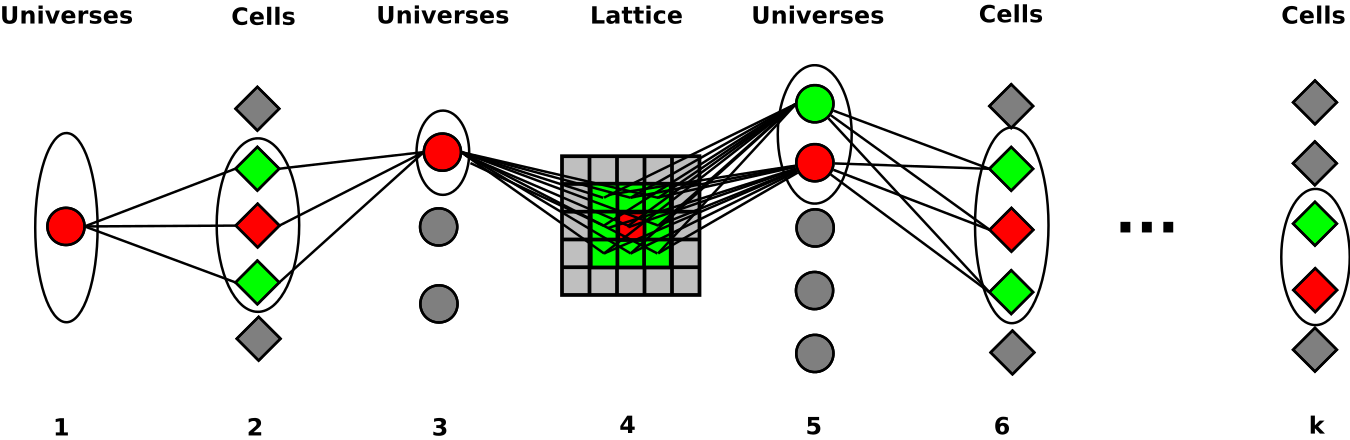
\includegraphics[width=0.8\linewidth]{figures/lns-k-partite-graph}
  \caption{A $k$-partite graph created by the OpenCG LNS algorithm.}
  \label{fig:lns-k-partite-graph}
\end{figure*}

%%%%%%%%%%%%%%%%%%%%%%%%%%%%%%%%%%%%%%%%%%%%%%%%%%%%%%%%%%%%%%%%%%%%%%%%%%%%%%%
\subsubsection{Flux-Weighted MGXS}
\label{subsubsec:lns-math}

Like the degenerate and null schemes, the LNS spatial homogenization scheme uses a single MC calculation of the complete heterogeneous geometry to generate MGXS for all materials. The MGXS are averaged across all pin instances with the same LNS identifier. Like the null and degenerate schemes, spatial self-shielding effects experienced by non-fissile spatial zones are averaged across the entire geometry. 

The LNS spatially-homogenized MGXS are computed as a flux-weighted average rather than as the geometric average of the MGXS in each pin instance. The reaction rates and fluxes for each fuel pin instance with the same LNS identifier are summed together and then divided to compute an average MGXS weighted by the relative flux in each pin instance. Unlike a geometric average of MGXS across pin instances, the flux-weighted average MGXS preserve global reaction rates.

% The MGXS were tallied separately for each instance of fissile material zones using OpenMC's distributed cell tallies. 

In order to formally express the flux weighted-average approach, it is useful to first define the microscopic MGXS $\hat{\sigma}_{x,i,k,g}$ estimated from MC tallies for reaction $x$, nuclide $i$, spatial zone $k$ and energy group $g$,

\begin{equation}
\label{eqn:general-micro}
\hat{\sigma}_{x,i,k,g} = \frac{\langle \sigma_{x,i}, \psi \rangle_{k,g}}{\langle \psi \rangle_{k,g}}
\end{equation}

\noindent where the angle bracket notation $\langle \cdot , \cdot \rangle$ represents an inner product over incoming and/or outgoing energy, space, and angle. In particular, subscript $k$ refers to a volume integral over $V_{k}$ for some region of space $k$ for spatial homogenization, and subscript $g$ corresponds to an integral over energies with $E \in [E_{g}, E_{g-1}]$ for energy condensation. The inner product of the spatially-homogenized and energy-integrated scalar flux with unity is simplified as $\langle \psi \rangle_{k,g} \equiv \langle \psi, \mathbb{1} \rangle_{k,g}$ in \autoref{eqn:general-micro}.

In this context, the index $k$ of $K$ total spatial zones refers to a particular instance of a fuel pin. The LNS algorithm represents a function $S(k)$ which assigns an identifier $m$ to each fuel pin instance based on its neighbors. The set $\mathbb{S}_{m}$ encapsulates all instances $k$ with the same LNS identifier $m$:

\begin{equation}
\label{eqn:lns-set}
\mathbb{S}_{m} = \left\{1 \le k \le K \;\;\; : \;\;\; S(k) = m\right\}
\end{equation}

LNS homogenization computes a single set of MGXS for the fuel pin instances in each set $k \in \mathbb{S}_{m}$ classified by the LNS algorithm. This is a specialization of \autoref{eqn:general-micro} with flux-weighted summations of the reaction rates and flux tallies in each pin instance:

\begin{equation}
\label{eqn:lns-micro}
\hat{\sigma}_{x,i,m,g} = \frac{\displaystyle\sum\limits_{k=1}^{K}\mathbb{1}_{\mathbb{S}_{m}}(k) \langle \sigma_{x,i}, \psi \rangle_{k,g}}{\displaystyle\sum\limits_{k=1}^{K}\mathbb{1}_{\mathbb{S}_{m}}(k) \langle \psi \rangle_{k,g}}
\end{equation}

\noindent where the indicator function $\mathbb{1}_{\mathbb{S}_{m}}(k)$ is equal to 1 if $k \in \mathbb{S}_{m}$ and 0 otherwise. The flux-weighted average is similarly applied to the MC tallies for each type of MGXS, including total, capture and fission production cross sections, scattering matrices and the fission spectrum.
